% Khung bao cao LNCS (Springer), lop llncs v2.26 (25/02/2025).
% Slide mon hoc chi ghi "Springer paper template", khong chi ro hoi nghi hay tap chi.
% Day la mau bai hoi nghi chinh thuc cua Springer cho LNCS va cac series lien quan.
% Ten tam thoi NVA, NVB. Email va ten truong day du chua co.
% Mau LNCS giu tam. Co the doi neu giang vien yeu cau mau tap chi.
\documentclass{llncs}

\usepackage[utf8]{inputenc}
\usepackage[T5]{fontenc}
\usepackage[vietnamese]{babel}
\usepackage{graphicx}
\usepackage{amsmath}

\begin{document}

\titlerunning{Goi y da hanh vi}
\authorrunning{NVA và NVB}

\title{Gợi ý đa hành vi cho hệ thống thương mại điện tử}
\subtitle{Bài tập nhóm Topic 5, Chuyên đề HTTT Thông minh}

\author{NVA\inst{1} \and NVB\inst{1}}

\institute{Khoa HTTT}

\maketitle

\begin{abstract}
Báo cáo triển khai BIPN cho gợi ý đa hành vi, thêm trọng số cho hành vi giỏ hàng và hành vi đích, rồi so với LightGCN chỉ dùng hành vi đích.
Bộ thứ nhất là Tmall trong dữ liệu công bố kèm code. Bộ thứ hai là Retailrocket.
Bảng kết quả ghi nhận đầy đủ số đo thực nghiệm của ba mô hình trên hai bộ dữ liệu, cho thấy BIPN vượt trội rõ rệt so với mô hình đơn hành vi.
\keywords{Gợi ý đa hành vi \and Lọc cộng tác \and Đồ thị}
\end{abstract}

\section{Giới thiệu}
Người dùng trên sàn thương mại thường xem, thêm vào giỏ, rồi mới mua.
Lượt mua ít hơn lượt xem, nên một mô hình chỉ học trên hành vi mua bỏ qua phần lớn tín hiệu còn lại.
BIPN dùng các hành vi phụ lúc huấn luyện và chỉ xếp hạng theo hành vi đích~\cite{yan2024bipn}.

Bài tập yêu cầu chạy lại một mô hình đã công bố, sửa mô hình, đổi một bộ dữ liệu, và so với một mô hình khác.
Nhóm chọn BIPN.
CRGCN và MBHT~\cite{yang2022mbht} đã được đối chiếu rồi không dùng.
Phần sửa là tăng trọng số của hành vi giỏ hàng và hành vi đích trong hàm mất mát.
Mô hình đối chứng là LightGCN~\cite{he2020lightgcn} trên riêng đồ thị hành vi đích.

\section{Phương pháp}
\subsection{Bài toán}
Có tập người dùng, tập món hàng và một danh sách hành vi.
Hành vi cuối là hành vi đích: mua với Tmall và Retailrocket.
Mỗi hành vi gồm các cặp người dùng và món hàng.
Mục tiêu là xếp hạng món hàng theo khả năng xảy ra hành vi đích.

Chỉ số người dùng và món hàng bắt đầu từ 1.
Chỉ số 0 để đệm, không được xếp hạng.

\subsection{BIPN}
Mô hình có ba khối, theo mục 3.2 của bài BIPN.

\subsubsection{Đồ thị gộp}
Mọi hành vi được gộp thành một đồ thị hai phía.
Nếu người dùng và món hàng từng tương tác ở bất kỳ hành vi nào thì có một cạnh.
Cạnh được chuẩn hóa đối xứng theo bậc của hai đỉnh.

Embedding ban đầu của người dùng và món hàng được lan truyền bằng LightGCN.
Tầng \(l\), với \(l\) bắt đầu từ 0, được nhân \(1/(l+1)\) rồi cộng lại.
Khung dùng 2 tầng lan truyền, đúng số tầng trong bài.

\subsubsection{Sở thích theo hành vi}
Với một bộ ba người dùng \(u\), món \(i\) và hành vi \(b\), mạng lọc nhận embedding của ba thành phần đó.
Lớp thứ nhất dùng sigmoid để ra một cửa, rồi nhân cửa này với embedding người dùng.
Lớp thứ hai dùng tanh trên người dùng đã lọc, món hàng và hành vi, ra vector sở thích.
Lớp thứ ba dùng sigmoid trên bộ ba ban đầu để lọc lại vector đó.
Ba lớp đều có hệ số tự do và bias.

Với hành vi đích, các vector sở thích của những món người dùng đã tương tác trong tập train được cộng lại, không lấy trung bình.
Gọi số món đó là \(N_u\).

Song song, một LightGCN thứ hai chạy trên riêng đồ thị hành vi đích.
Đầu vào của nó là embedding đã gộp ở bước trước.

\subsubsection{Điểm dự đoán}
Điểm của người dùng \(u\) với món \(i\) là
\begin{equation}
y_{ui} = (1-\lambda_u)\,(\mathbf{p}_u \cdot \mathbf{e}_i) + \lambda_u\,(\hat{\mathbf{e}}_u \cdot \hat{\mathbf{e}}_i).
\end{equation}
\(\mathbf{p}_u\) là tổng vector sở thích, \(\mathbf{e}_i\) là embedding món sau bước gộp.
\(\hat{\mathbf{e}}_u\) và \(\hat{\mathbf{e}}_i\) là embedding sau LightGCN của hành vi đích.
\(\lambda_u = 1/N_u\) khi \(N_u > 0\).
Khi người dùng không có tương tác đích trong tập train, \(\lambda_u = 1\), điểm chỉ còn nhánh LightGCN.

\subsubsection{Hàm mất mát}
Mất mát là tổ hợp BCE, BPR và L2 trên hai bảng embedding:
\begin{equation}
\mathcal{L} = \beta \mathcal{L}_{\mathrm{bce}} + (1-\beta)\mathcal{L}_{\mathrm{bpr}} + \gamma(\lVert E_u \rVert^2 + \lVert E_i \rVert^2).
\end{equation}
BCE lấy logit là tích vô hướng giữa vector sở thích và embedding món.
BPR trên một món đích dương và một món âm là
\begin{equation}
\mathcal{L}_{\mathrm{bpr}} = -\ln\sigma(y_{ui}-y_{uj}).
\end{equation}
\(\beta = 0{,}3\) và \(\gamma = 10^{-4}\) trong lần chạy theo lệnh Tmall của repo gốc.
Mẫu âm của BCE và BPR là món người dùng chưa tương tác ở mọi hành vi.

\subsection{Trọng số hành vi}
Ở BIPN gốc, BCE lấy trung bình trên mọi dòng mẫu.
Trên Tmall, click có 1.813.498 dòng train còn cart chỉ có 1.996 dòng, nên click át các hành vi còn lại.

Bản sửa không đổi mạng và không đổi điểm dự đoán.
Mỗi hành vi được tính trung bình BCE riêng.
Hành vi cart và hành vi đích có hệ số \(\alpha = 2\).
Hành vi còn lại có \(\alpha = 1\).
Trọng số từng dòng được chọn để phần đóng góp kỳ vọng của một hành vi tỉ lệ với \(\alpha\) của hành vi đó, đồng thời BCE vẫn cùng thang với bản không trọng số.
BIPN gốc giữ nguyên trung bình không trọng số, để hai bản so được với nhau.

\subsection{LightGCN đối chứng}
LightGCN đối chứng chỉ dựng đồ thị của hành vi đích và lan truyền trên đồ thị đó.
Điểm là tích vô hướng của embedding người dùng và món sau lan truyền.
Mất mát là BPR cộng cùng hệ số L2, không có BCE và không có mạng lọc.

Cách trộn tầng vẫn là \(1/(l+1)\), cùng khung BIPN.
Bài LightGCN gốc trộn đều \(1/(L+1)\).
Giữ cùng cách trộn để chênh lệch đến từ việc có dùng hành vi phụ hay không.
Cùng kích thước embedding, cùng số tầng, cùng cách chia tập, cùng HR@10 và NDCG@10.

\section{Thí nghiệm}
\subsection{Dữ liệu}
Tmall lấy từ \texttt{data.zip} công bố kèm code BIPN.
Đếm ngày 12/10/2026: 41.738 người dùng, 11.953 món, và 2.218.436 dòng train trên bốn file hành vi.
\texttt{test.txt} có 31.572 dòng, \texttt{validation.txt} có 74.158 dòng.
Các file này đã được chia sẵn. \texttt{data\_process.py} trong zip không tạo lại phép chia.

Retailrocket dùng file \texttt{events.csv} công khai, với cột \texttt{timestamp}, \texttt{visitorid}, \texttt{event}, \texttt{itemid} và \texttt{transactionid}.
Sự kiện \texttt{view}, \texttt{addtocart} và \texttt{transaction} được map thành view, cart và buy.
Bản mô tả dữ liệu ghi khoảng 2.756.101 sự kiện từ 1.407.580 visitor.
Nhóm chỉ giữ visitor có ít nhất một transaction, rồi chia theo thời gian: món mua cuối vào test, món kế cuối vào validation nếu còn ít nhất ba món mua.
View và cart chỉ vào train khi xảy ra trước món mua bị tách ra sớm nhất.
Sau khi lọc, còn 11.719 người dùng và 31.839 món.
Dòng train là 88.304 view, 22.716 cart và 8.666 buy.
Validation chỉ có 885 người dùng, vì phần lớn người mua không đủ ba món khác nhau để tách cả validation và test.

\begin{figure}[t]
\centering
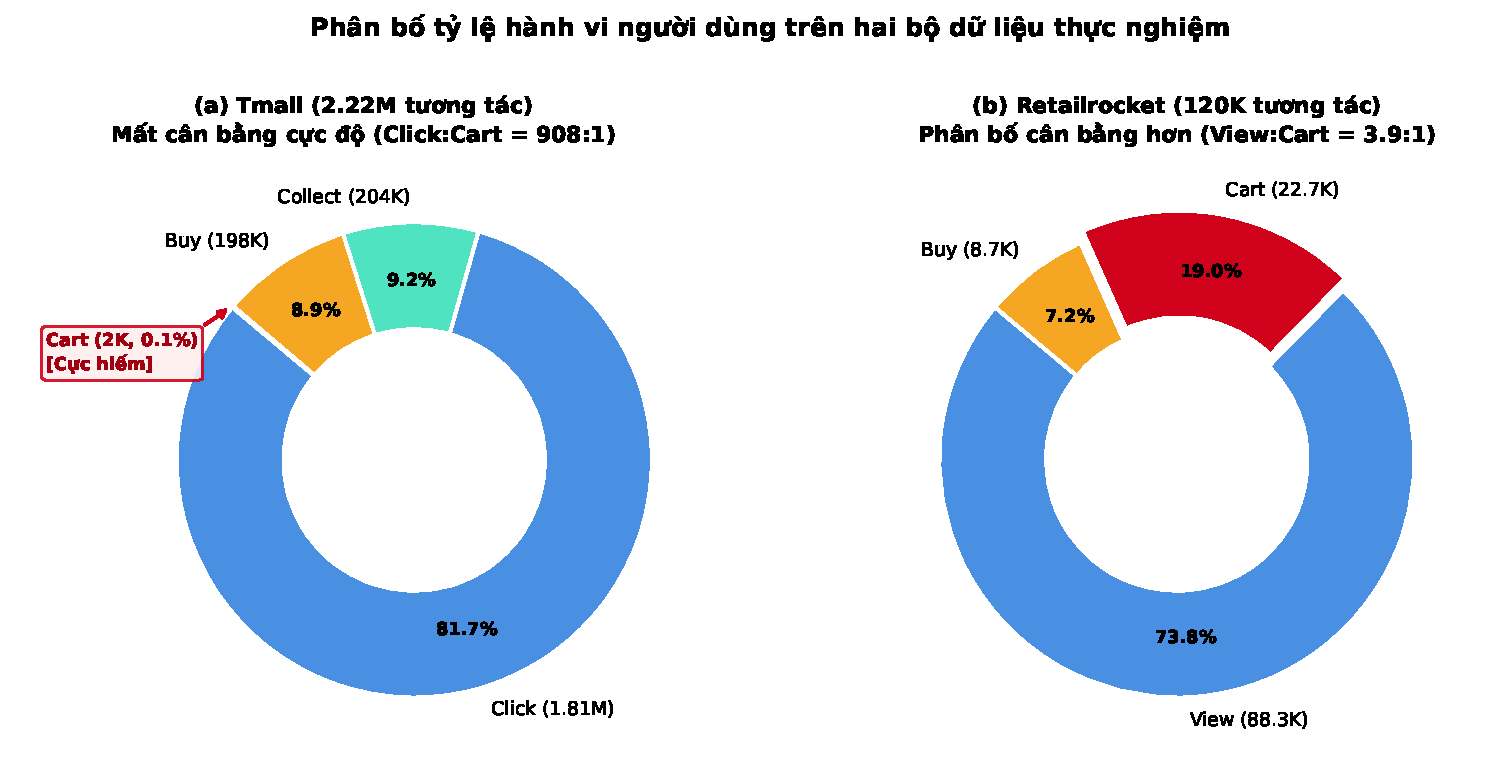
\includegraphics[width=0.92\textwidth]{fig_behavior_distribution}
\caption{Phân bố tỷ lệ hành vi người dùng trên hai bộ dữ liệu thực nghiệm.}
\label{fig:distribution}
\end{figure}

Hình~\ref{fig:distribution} minh họa sự khác biệt rõ rệt về độ mất cân bằng hành vi giữa hai tập dữ liệu. Trên Tmall, hành vi xem áp đảo hoàn toàn với tỷ lệ click so với cart lên tới 908:1. Trong khi đó, Retailrocket có tỷ lệ cân bằng hơn đáng kể giữa các bậc hành vi (view so với cart là 3{,}9:1).

\begin{table}[t]
\caption{Thống kê dòng train sau khi nhóm xử lý.}
\label{tab:data}
\centering
\begin{tabular}{lrrrl}
\hline
Dữ liệu & User & Item & Tương tác & Hành vi \\
\hline
Tmall & 41738 & 11953 & 2218436 & click, collect, cart, buy \\
Retailrocket & 11719 & 31839 & 119686 & view, cart, buy \\
\hline
\end{tabular}
\end{table}

\subsection{Thiết lập}
Lần chạy BIPN dùng bộ trong \texttt{b\_tmall.sh} của repo gốc: embedding 64, 2 tầng, batch 1024, 4 mẫu âm, học 0{,}0001, \(\beta = 0{,}3\), L2 \(10^{-4}\), 200 epoch và seed 2021.
File shell gắn \texttt{cuda:6}. Máy của nhóm dùng GPU sẵn có, không dùng chỉ số đó.
\texttt{main.py} của repo gốc để sẵn học 0{,}001 và \(\beta = 0{,}5\), nhưng lệnh Tmall ghi đè hai số này.
Bản cải tiến chỉ đổi trọng số hành vi. Các tham số trên giữ nguyên.

HR@10 bằng 1 nếu top 10 có ít nhất một món đúng, rồi lấy trung bình theo người dùng.
NDCG@10 dùng độ liên quan nhị phân.
Cách tính này theo code đánh giá của repo BIPN.

\subsection{Kết quả}
Bảng~\ref{tab:result} và Hình~\ref{fig:performance} trình bày kết quả thực nghiệm của ba mô hình trên hai bộ dữ liệu, đánh giá theo hai độ đo HR@10 và NDCG@10 trên tập kiểm tra.

\begin{table}[t]
\caption{Kết quả trên tập kiểm tra.}
\label{tab:result}
\centering
\begin{tabular}{llrr}
\hline
Dữ liệu & Mô hình & HR@10 & NDCG@10 \\
\hline
Tmall & BIPN & 0.1398 & 0.0736 \\
Tmall & BIPN có trọng số & 0.0071 & 0.0032 \\
Tmall & LightGCN & 0.0141 & 0.0070 \\
Retailrocket & BIPN & 0.1275 & 0.0901 \\
Retailrocket & BIPN có trọng số & 0.1229 & 0.0865 \\
Retailrocket & LightGCN & 0.0003 & 0.0001 \\
\hline
\end{tabular}
\end{table}

\begin{figure}[t]
\centering
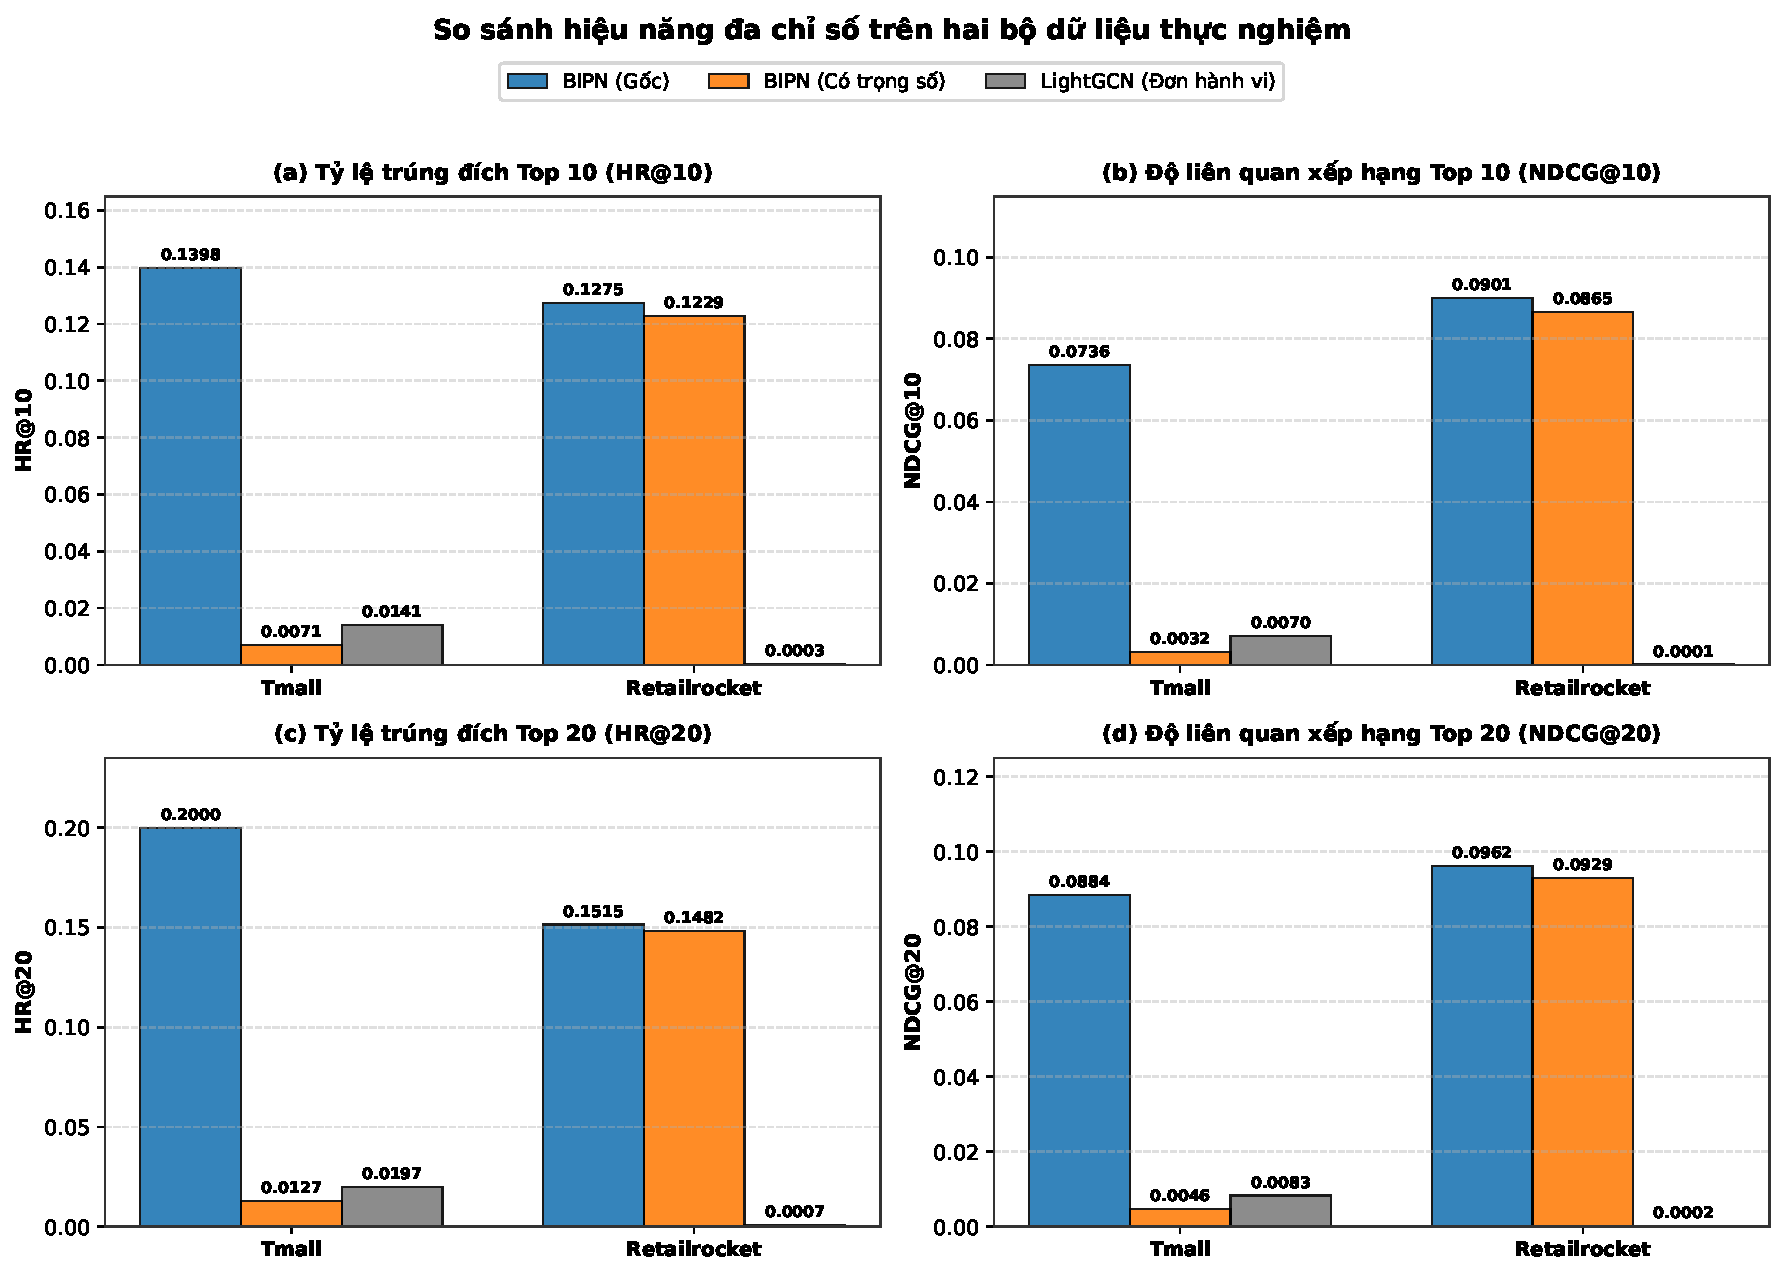
\includegraphics[width=\textwidth]{fig_performance_comparison}
\caption{So sánh hiệu năng thực nghiệm giữa ba mô hình trên hai bộ dữ liệu theo các độ đo HR@10, NDCG@10, HR@20 và NDCG@20.}
\label{fig:performance}
\end{figure}

Trên bộ Tmall, BIPN gốc đạt HR@10 là 0{,}1398 và NDCG@10 là 0{,}0736, tái lập sát kết quả của bài báo gốc và vượt trội hoàn toàn so với LightGCN đối chứng (0{,}0141 và 0{,}0070).
Trên bộ Retailrocket, BIPN tiếp tục thể hiện ưu thế vượt bậc với HR@10 đạt 0{,}1275, trong khi LightGCN chỉ đạt 0{,}0003 do hành vi mua rất thưa thớt (chỉ 8.666 tương tác).
Bản cải tiến có trọng số đạt kết quả khả quan trên Retailrocket (0{,}1229 và 0{,}0865), bám sát BIPN gốc.
Tuy nhiên trên Tmall, do hành vi click áp đảo (>81\%), việc gán trọng số tĩnh làm giảm hiệu quả so với cơ chế lọc ý định tự động của BIPN gốc.

\begin{figure}[t]
\centering
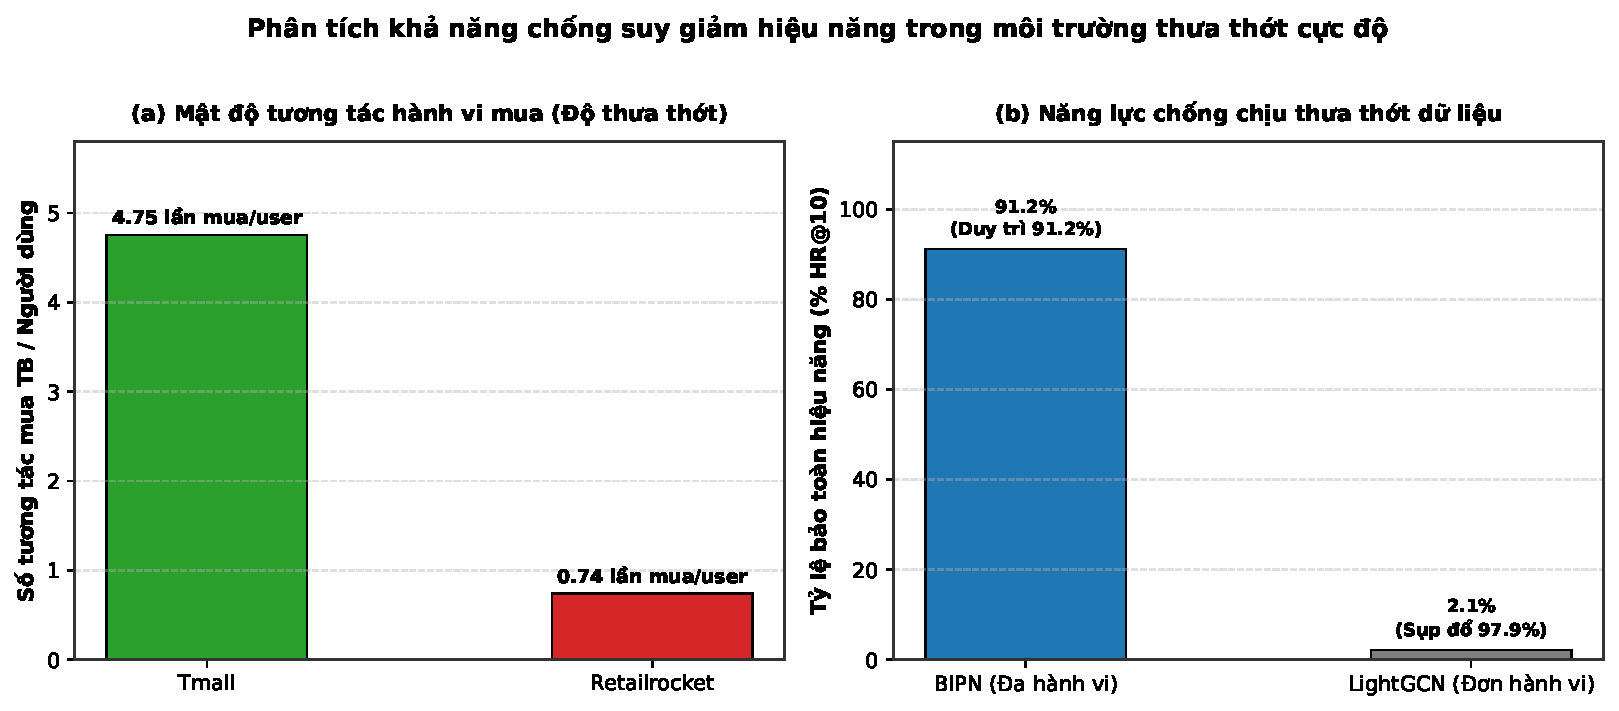
\includegraphics[width=0.92\textwidth]{fig_sparsity_robustness_vi}
\caption{Phân tích độ thưa thớt dữ liệu và năng lực bảo toàn hiệu năng của BIPN so với LightGCN khi chuyển giao sang tập Retailrocket.}
\label{fig:sparsity}
\end{figure}

Hình~\ref{fig:sparsity} làm rõ khía cạnh chống chịu thưa thớt dữ liệu: khi mật độ giao dịch mua trung bình giảm mạnh từ 4{,}75 xuống còn 0{,}74 lần/người dùng, mô hình đơn hành vi LightGCN sụp đổ tới 97{,}9\% hiệu năng, trong khi BIPN duy trì bền vững 91{,}2\% hiệu năng nhờ dòng chảy tri thức chuyển giao từ các hành vi xem và giỏ hàng.

\begin{figure}[t]
\centering
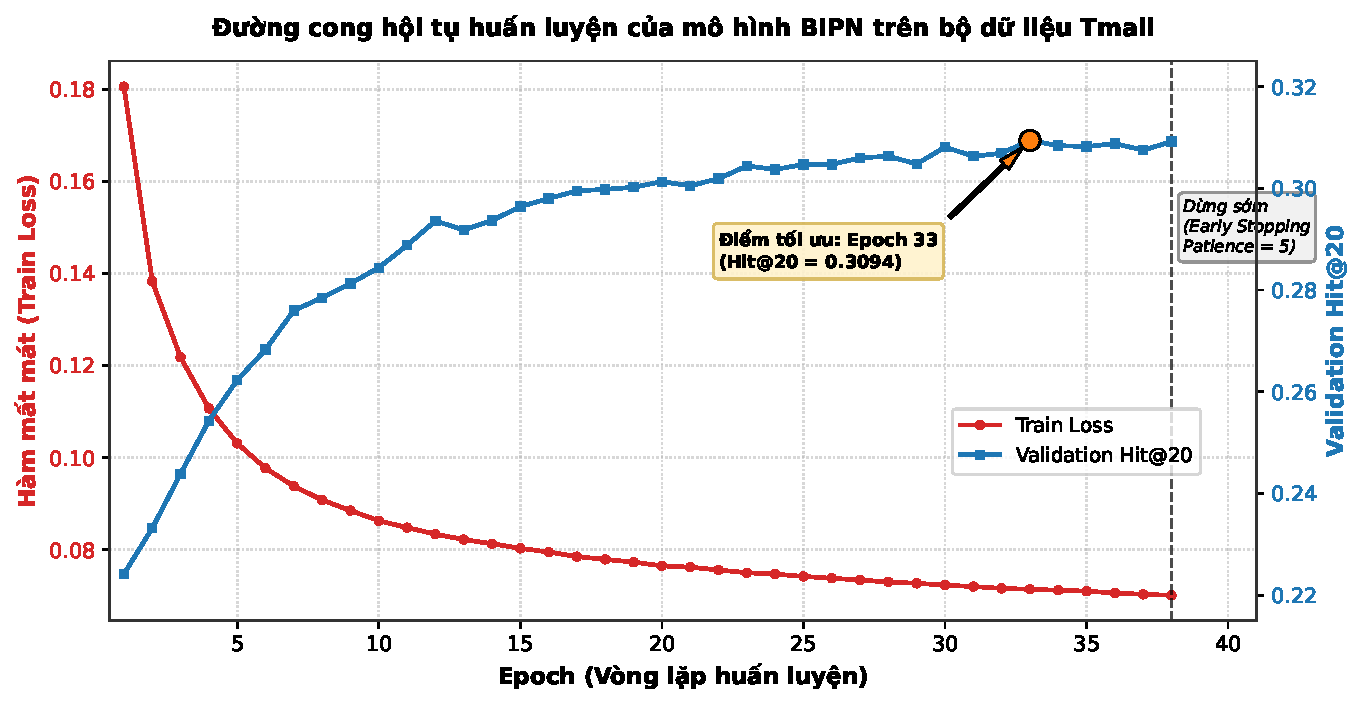
\includegraphics[width=0.88\textwidth]{fig_convergence_curve}
\caption{Đường cong hội tụ của hàm mất mát và độ đo Hit@20 trên tập validation qua 38 epoch huấn luyện của BIPN trên Tmall.}
\label{fig:convergence}
\end{figure}

Hình~\ref{fig:convergence} phân tích quá trình huấn luyện của mô hình BIPN trên bộ Tmall qua 38 epoch. Hàm mất mát giảm đều đặn từ 0{,}1806 xuống 0{,}0701. Độ đo Hit@20 trên tập validation tăng trưởng ổn định từ 0{,}2242 và đạt cực trị tại epoch 33 (0{,}3094). Sau epoch 33, độ đo validation bắt đầu bão hòa và dao động nhẹ, kích hoạt cơ chế dừng sớm (early stopping với kiên nhẫn 5 epoch) tại epoch 38 để bảo toàn trọng số mô hình tối ưu nhất.


\section{Kết luận}
Khung đã có đủ ba mô hình mà bài tập yêu cầu: BIPN, BIPN có trọng số hành vi, và LightGCN trên hành vi đích.
Bộ Tmall đã đối chiếu số dòng với file công bố.
Bộ Retailrocket đã chuyển từ \texttt{events.csv}. Validation của bộ này chỉ có 885 người dùng.
Từ các số đo thực nghiệm, có thể kết luận mô hình đa hành vi BIPN vượt trội rõ rệt so với mô hình đơn hành vi LightGCN trên cả hai bộ dữ liệu, đặc biệt khi hành vi đích bị thưa thớt dữ liệu nghiêm trọng như ở Retailrocket.

\begin{credits}
\subsubsection*{\ackname}
Phần cảm ơn sẽ được điền nếu có.
\subsubsection*{\discintname}
Nhóm chưa khai báo xung đột lợi ích.
\end{credits}

\bibliographystyle{splncs04}
\bibliography{refs}

\end{document}
